\chapter{Softwarearchitekturanalyse bestehender Programme}\label{Kap2}

    Analysemethoden der Informatik für Software sind in der Regel für die verschiedenen Design-Phasen entwickelt worden.
    Eine von mir durchgeführte Internet-Recherche ergab, dass sich Analyse-Tools und Methoden für bestehende Software vor
    allem darauf fokussieren, die Performance, Speichermanagement und Benutzererfahrung zu bewerten.
    Die Architektur einer Software spielt dabei eine untergeordnete Rolle.
    Für einen Nachfolger der Lagerverwaltung 3.0 soll jedoch zunächst ihre Softwarearchitektur untersucht werden.
    Die Performance und der Speicherverbrauch spielen für die $\mu$Plant eine untergeordnete Rolle.
    Eine Bewertung der Programmkomponenten sollt also anhand folgender Kriterien bewertet werden:

    \begin{itemize}
        \item Ihrem Nutzen für den Anwender
        \item Zuverlässigkeit im Betrieb
        \item Umgang mit erwartbaren Fehlern
    \end{itemize}

    Der Programmcode sollte zudem
    \begin{itemize}
        \item Leicht lesbar und verständlich,
        \item Zuverlässig und robust, und
        \item gut erweiterbar sein.
    \end{itemize}
    In einem C$\#$ Projekt sind GUI und Buisinesslogik in getrennten Dateien implementiert.
    XAML-Dateien gehören zu Microsofts .NET Plattform. 
    Ihr Dateiformat ähnelt denen von XML-Dateien. 
    Sie legen fest wie das GUI gerendert wird und werden im integrierten Editor der Visual Studio IDE bearbeitet.
    .XAML.cs Dateien implementieren die Controller-Logik des XAML-Inhalts. 
    Ihre Programmiersprache ist C$\#$.

    Am Beispiel des Startbildschirms des Programms \glqq Lagerverwaltung 3.0\grqq wird der Programmaufbau geschildert.
    Aufgrund der Komplexität und des fehlenden Mehrwerts wird weiteren Verlauf dieser Arbeit darauf verzichtet.
    Aus dem gleichem Grund wird auf die detaillierte Beschreibung der Funktionsweise von grafischen ELementen ihrer Events
    sowie ihrer Eventhandler verzichtet.

    In den erstellen Klassendiagrammen ist gut ersichtlich, welche Klassen Events nutzen.
    Sie erben von der Klasse \verb|INotifyPropertyChanged|.
    Die Klasse ist ein Interface der .NET Plattform und wird immer dann eingesetzt, wenn eine GUI-Komponente über eine Änderung
    informiert werden soll. Sie wird im Allgemeinen dafür benutzt um das GUI mit dem hinterlegten Datenmodell zu verknüpfen.

    Wenn diese Klasse implementiert wird, muss die Methode \verb|OnPropertyChanged| überschrieben werden, die immer dann aufgerufen wird,
    wenn sich ein Wert ändert. 
    \clearpage

    \section {Lagerverwaltung 3.0}

    Wie in dem einleitenden Abschnitt angekündigt wird zunächst der grundlegende Aufbau des Programms beschrieben.\\

    Die Datei \verb|App.xaml| ist der Einstiegspunkt des Programms.
    In ihr wird ein Objekt der Application-Klasse mit allen benötigten Ressourcen erzeugt.
    Als Start URL ist \verb|MainWindow.xaml| angeben.\\
    In der Datei ist beschrieben, wie der Startbildschirm gerendert wird.

    Zunächst wird ein Banner gerendert, bestehend aus dem Titel des Programms, dem Logo des Instituts und der $\mu$Plant
    (Siehe Abb.\ref{fig:figure} Bereich \glqq A\grqq).
    Es werden außerdem alle benötigten Datenobjekte erzeugt.
    Sie lassen sich wie folgt einteilen:
    
    \begin{itemize}
        \item Objekte und Variablen, die dem Lager zugeordnet sind:
            \begin{itemize}
                \item Ein Objekt \verb|inventory| der Klasse \verb|Inventory| für das Inventar mit \verb|null| initialisiert.
                \item Ein Objekt \verb|storageMatrix| von der Klasse \verb|PalletMatrix| erzeugt.
                \item Ein Object \verb|commissionMatrix| von der Klasse \verb|PalletMatrix| erzeugt.
                \item Ein Objekt \verb|mobileRobot| von der Klasse \verb |MobileRobot| erzeugt.
                \item Außerdem eine Variable \verb|lastCupRead| vom Datentyp \verb|ushort| (16-Bit-Ganzzahl, vorzeichenlos) mit 0 initialisiert.
            \end{itemize}
            \item Objekte und Variablen initialisiert, die dem ABB Controller zugeordnet sind:
            \begin{itemize}
                \item Ein Objekt \verb|commands| von der Klasse \verb|controllerCommandList|.
                \item Ein Objekt \verb|controllerProperties| von der Klasse \verb|RobotControllerProperties|.
                \item Ein Objekt \verb|controllerBase| von der Klasse \verb|RobotControllerBas|, mit dem Initialisierungswert \verb|null|.
                \item Ein Objekt \verb|controllerSim| von der Klasse \verb|RobotSimulator|.
            \end{itemize}
    \end{itemize}

    Im Constructor der Klasse \verb|MainWindow| werden zudem der ModBus und der Roboter Controller initialisiert
    und ihre GUI-Elemente gerendert (Abb.\ref{fig:figure} Bereiche \glqq B\grqq{} und \glqq C\grqq).
    
    Die Produktliste wird aus der Datei \verb|Produkte.db| geladen und gerendert (Abb.\ref{fig:figure} Bereich \glqq D\grqq).
    
    Daten des Lagers und des mobilen Roboters sowie die Kommissionsdaten werden aus der Datei \verb|CommissionData.db|
    geladen und anschließend das Inventar gerendert (Abb.\ref{fig:figure} Bereich \glqq E\grqq{}  und \glqq G\grqq).
    
    Bereich \glqq F\grqq{} ist der Eventlog der Anwendung, dort werden alle Ereignisse der Software als Text angezeigt.
    Das können Fehler sein aber auch Fortschritte im Programmablauf.

    Im mittleren Bereich ist die Anordnung von Roboter, Andockstation und Kommissioniertisch symbolisiert.
    Der \glqq Start\grqq -Knopf startet den Automatikbetrieb.
    Nach dem Start der Automatik kann der selbe Knopf zum Stoppen des Automatikbetriebs verwendet werden.

    Wenn keine Verbindung zum Modbus hergestellt werden kann, wird dem Benutzer angeboten die Vorgänge zu simulieren.
    Im Klassendiagramm Abb.\ref{fig:figure2} wird jedoch schnell deutlich, dass dieser Simulationsbetrieb nicht für einen Testbetrieb
    geeignet ist, da dazu eine ganz andere Klasse verwendet wird.

    Im Bereich \glqq Mobile Robot\grqq{} wird nach erfolgreichem Andocken das erkannte Produkt angezeigt.
    Dem Bediener wird hier angeboten die Daten manuell zu manipulieren oder Details ein- bzw. auszublenden.

    Im Bereich \glqq Workbench\grqq{} werden bis zu zwei Paletten mit ihrem Inhalt gerendert.
    Auch hier wird dem Benutzer angeboten, die Daten per Hand zu manipulieren.

    Im Folgenden werden die wichtigsten Klassenstrukturen beschrieben.
    Auf die Beschreibungen von Hilfsklassen und solche, die für die .NET Plattform oder die Programmiersprache C$\#$ spezifisch sind, wird verzichtet.

    \begin{figure}[h]
        \caption[Ansicht des Startbildschirms]
        {\small Startbildschirm der Anwendung, zur besseren Beschreibung sind die Bedienbereiche rot umrandet und mit
        Buchstanben gekennzeichnet}\label{fig:figure}
        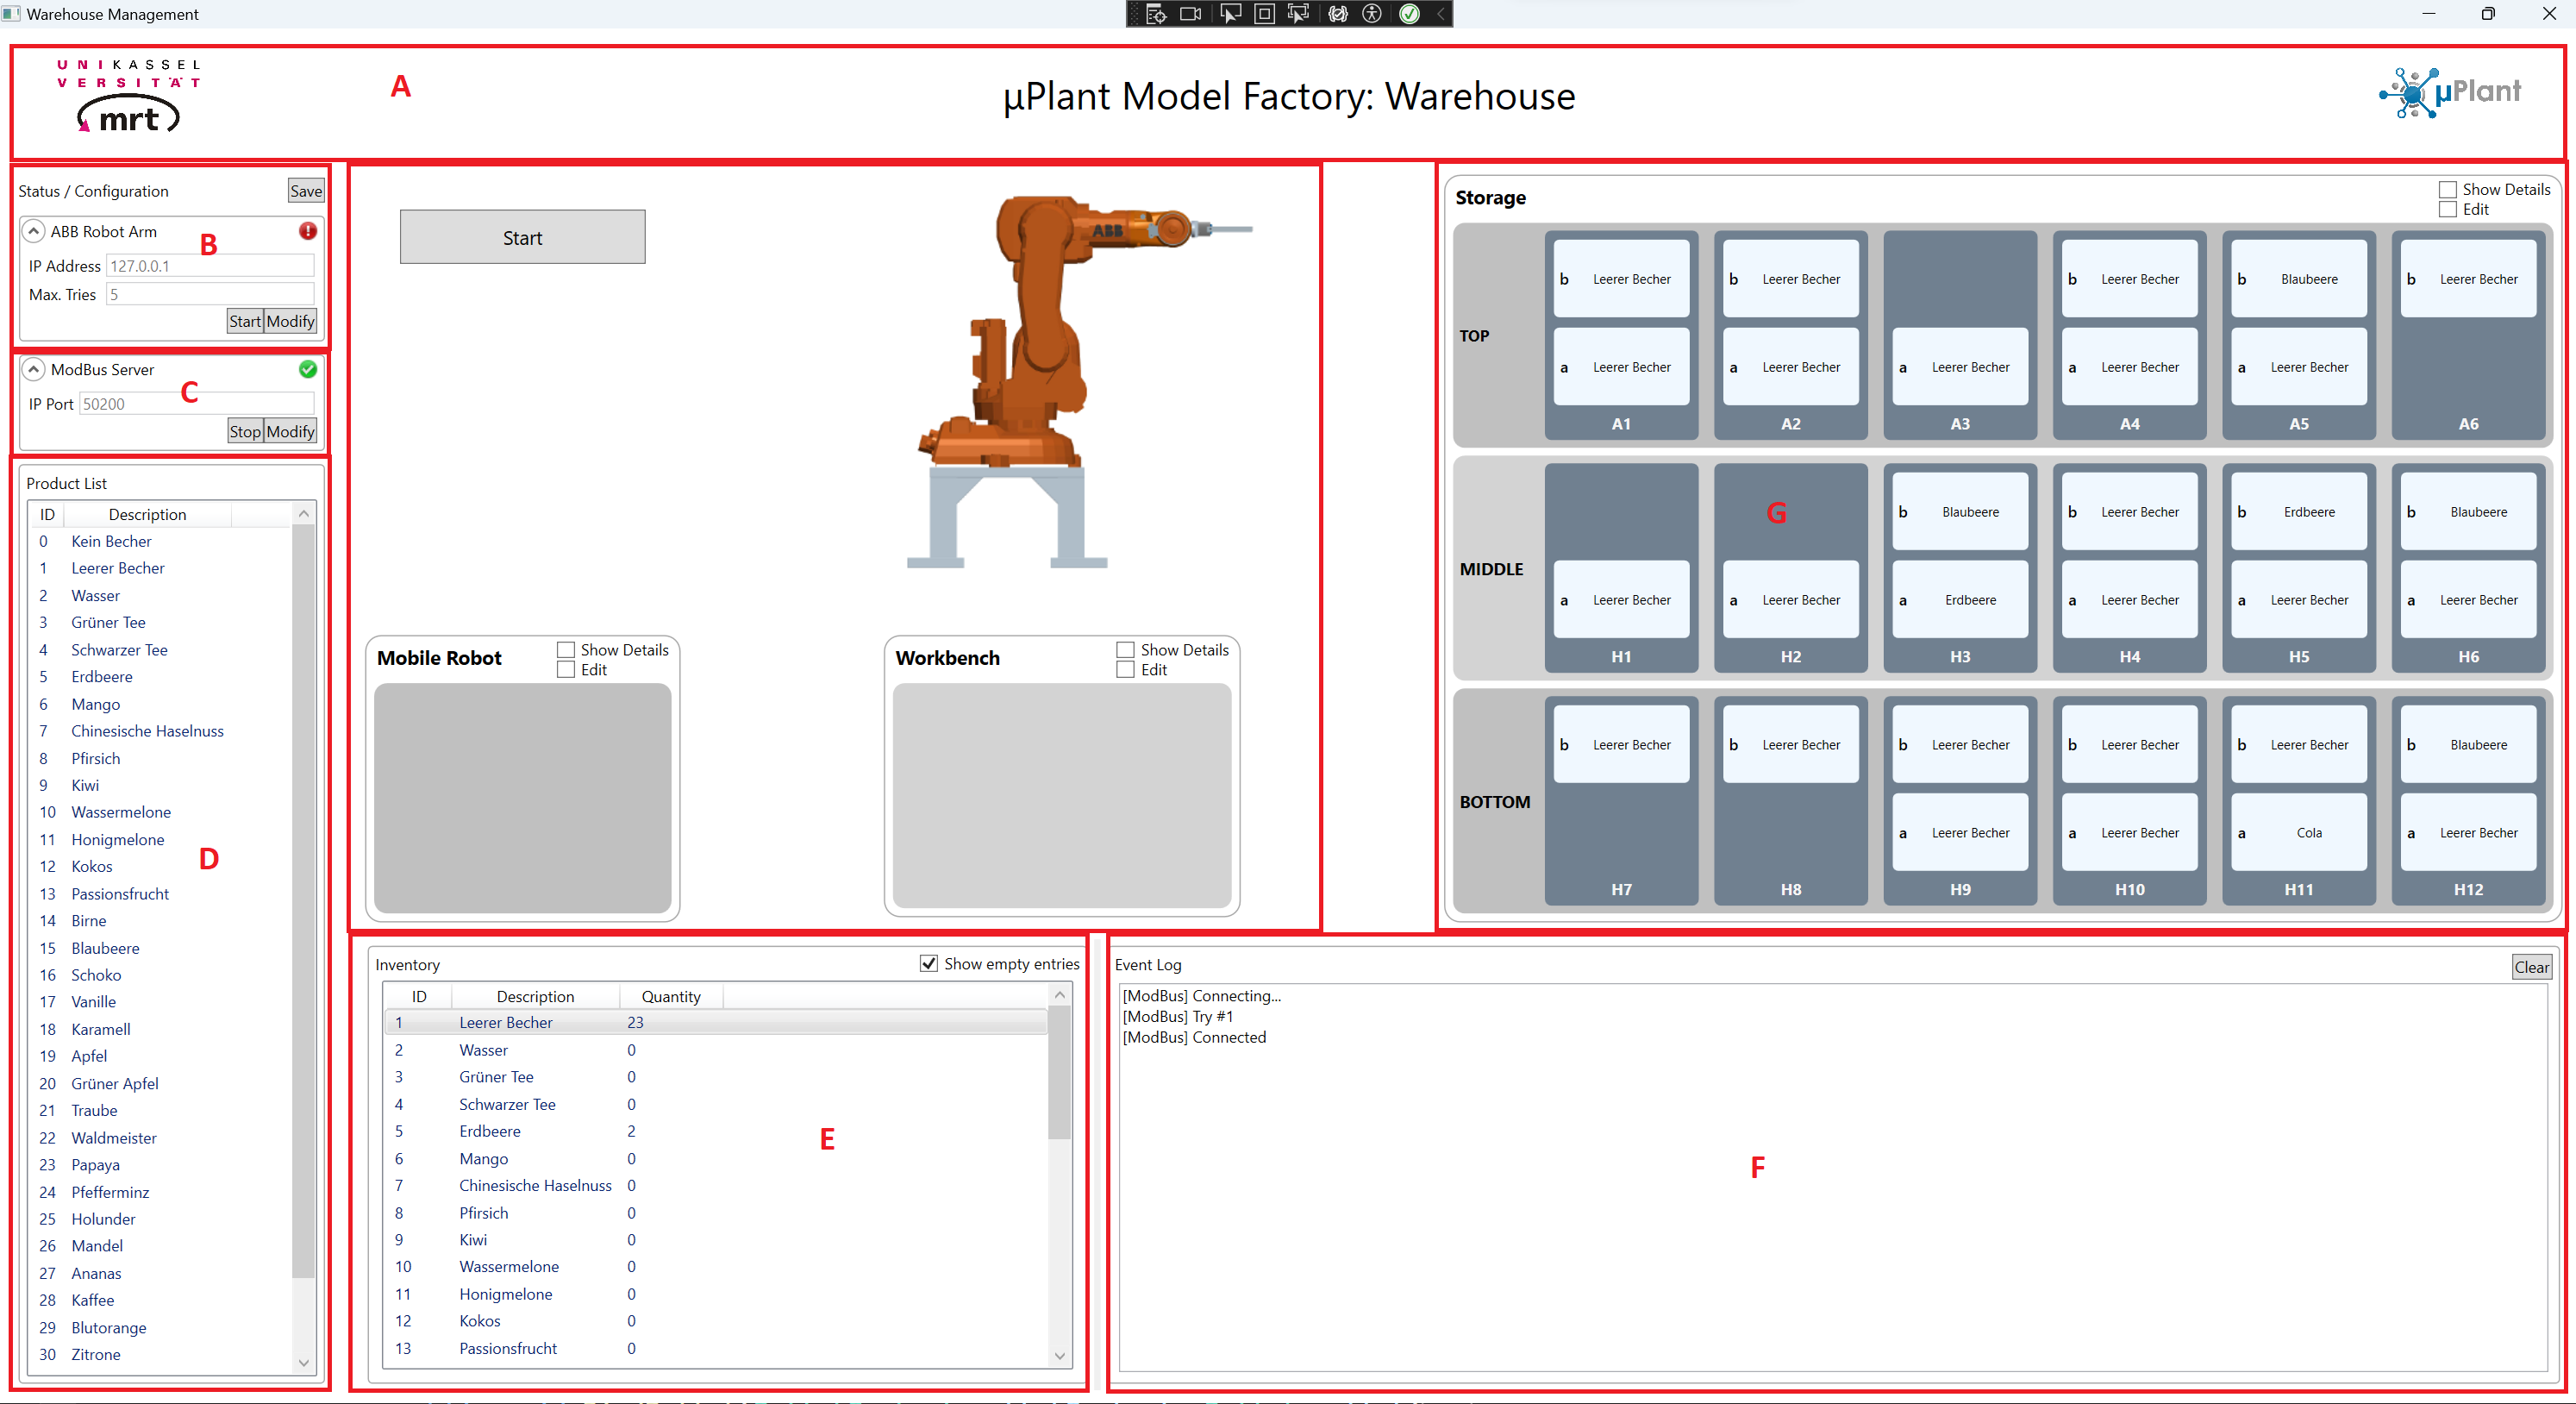
\includegraphics[width = \textwidth ]{Bilder/LV_Startbildschirm}
        \centering
    \end{figure}

    \subsection{Klassenstruktur des Datenmodells}\label{Datenmodell}

    Die bestehende Software dient dazu Lagerpakete vom mobilen Roboter auf die Werkbank oder ins Lager zu bewegen.
    Oder alle möglichen Kombinationen davon. 
    Ein Lagerpaket ist einer der nachfolgenden Varianten:
    \begin{itemize}
        \item Ein Becher
        \item Eine leere Palette
        \item eine Palette mit einem oder zwei Bechern
    \end{itemize}
    
    Der Programmierer hat sich diese Struktur angeeignet und in der Datenmodellierung umgesetzt.
    In Abb.\ref{fig:figure2} ist gut ersichtlich, dass die Klasse \verb|StorageElementBase| an die Klassen \verb|Cup| und \verb|Pallet|
    vererbt (schmale Linie mit leerem Pfeil, in Anlehnung an UML). Eigenschaften, die sowohl Palette als auch den
    Becher betreffen, sind in dieser Klasse implementiert.

    Weiterhin findet sich das Lager als eigene Klasse \verb|Inventory| und der mobile Roboter als \verb|MobileRobot| wieder.
    Die \verb|Inventory|-Klasse ist jedoch nicht das Lager im Sinne von Abb.\ref{fig:figure2} Bereich \glqq G\grqq, sondern auf die Liste in
    Bereich \glqq E\grqq.\\

    \begin{figure}
        \caption[Klassendiagramm Datenmodells ]
        {\small Klassendiagramm der MainWindow-Klasse mit vererbenden- und Datenmodell - Klassen }\label{fig:figure2}
        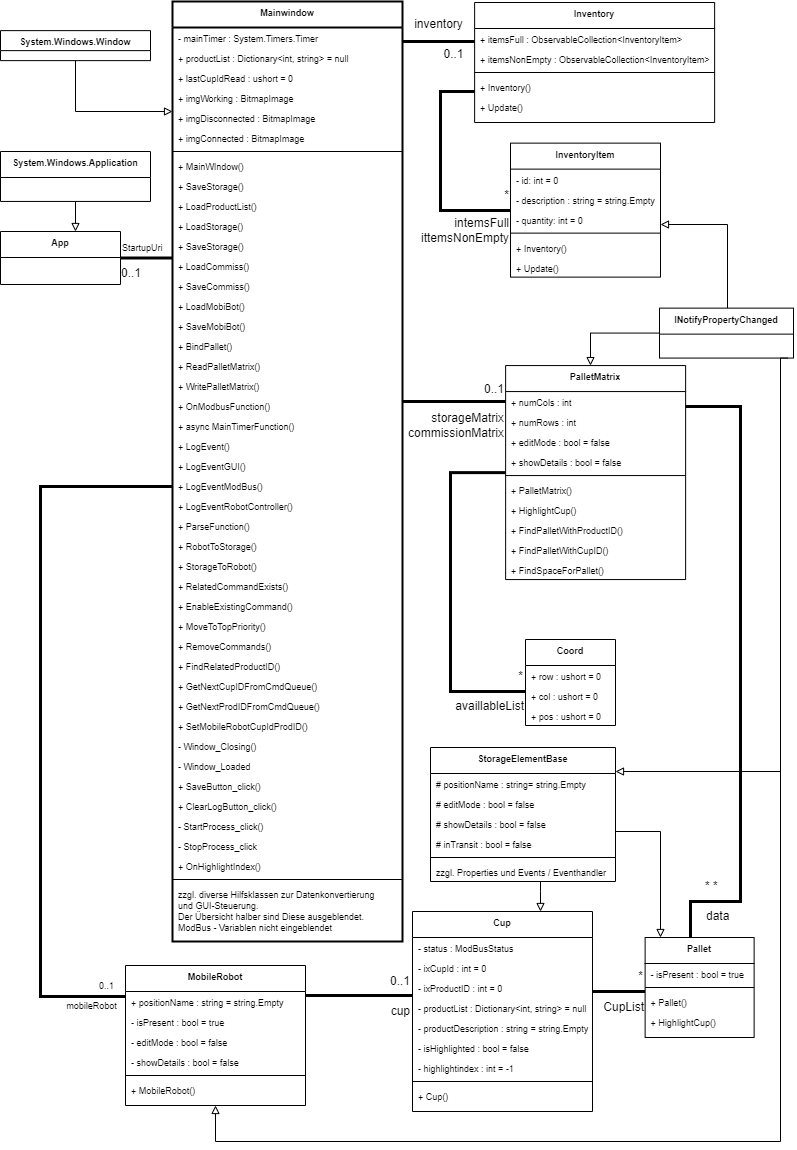
\includegraphics[width = \textwidth ]{Bilder/LV_Klassendiagramm_Datenmodell}
        \centering
    \end{figure}
    \clearpage

    Zentrales Element ist die \verb|MainWindow| Klasse.
    Sie implementiert eigentlich die Interface-Klasse \verb|System.Windows.Window|.
    Der Programmierer hat sie allerdings auch als Daten-Hub verwendet.
    
    Wie zu Beginn des Abschnitts geschildert werden beim Rendern des Fensters alle benötigten Datenobjekte erzeugt oder aus Dateien geladen.

    \begin{itemize}
        \item In der Klasse \verb|Inventory| wird der Inhalt der Datei \verb|Produkte.db| in zwei Listen geladen, sodass
        eine Liste mit lagernden Produkten und eine vollständige Produktliste gespeichert werden.
        Eine Instanz \verb|inventory| wird zur Laufzeit erzeugt. Wenn die Dateien \verb|Produkte.db| und
        \verb|StorageData.db| zu dem Zeitpunkt nicht verfügbar ist, stürzt das Programm ab.
        \item In der Klasse \verb|PalletMatrix| wird die Datei \verb|StorageData.db| bzw. \\ \verb|CommissionData.db|
        geladen um einen zweidimensionalen Array \verb|data| zu erzeugen.
        Jedes Array-Element ist ein Objekt der Klasse \verb|Pallet| und enthält eine Liste \verb|CupList| von Objekten
        der Klasse \verb|Cup|.
        Diese Struktur wird dazu verwendet, um das reale Lager zu visualisieren.
        Zur Laufzeit werden zwei Objekte der Klasse \verb|PalletMatrix| erzeugt:
        \begin{itemize}
            \item \verb|storageMatrix| bildet das Datenmodell um die Visualisierung in Abb.\ref{fig:figure2} Bereich \grqq G\glqq{} zu realisieren.
            \item \verb|commissionMatrix| bildet das DatenModell für die Visualisierung des mobilen Roboters und der
            Workbench.
        \end{itemize}
    \end{itemize}
\newpage
    \begin{figure}
        \caption[Klassendiagramm ABBRobotics Controller ]
        {\small Klassendiagramm der MainWindow-Klasse mit Klassen aus dem ABBRobotics Controllerframework. }\label{fig:figure3}
        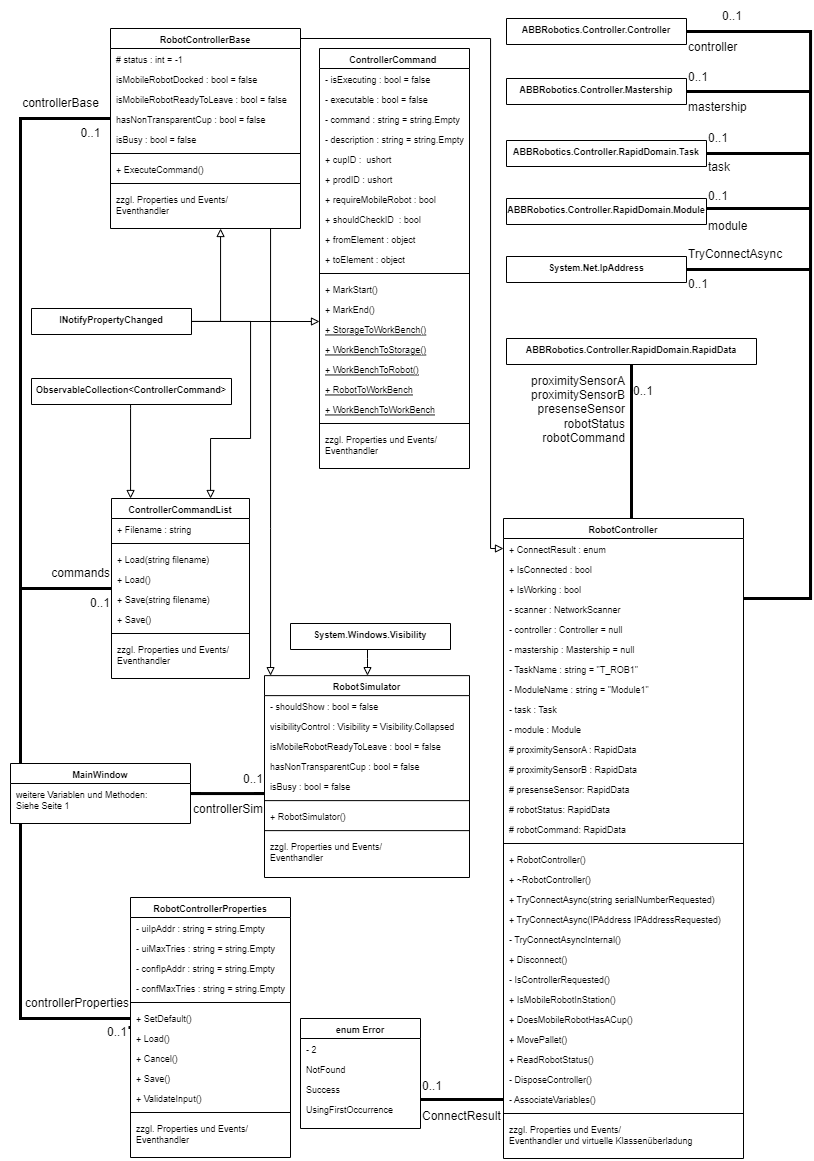
\includegraphics[width = \textwidth ]{Bilder/LV_Klassendiagramm_ABBController}
        \centering
    \end{figure}

\subsection{Klassenstruktur zur Steuerung des ABB Industrieoboter IRB 140}\label{ABBKlassen}

Um dem Industrieroboter ABB IRB 140 Kommandos zu senden, muss das Programm mit der Steuerung IRC5 kommunizieren.
Die Steuerung ist Baujahr 1991 und hat eine Firmware \glqq RobotWare 5.15.1004.01\grqq{} installiert.
Die Kommunikation erfolgt über ein verschlüsseltes TCP/IP Protokoll. 

Im Programmcode finden sich dazu wie in Abb.\ref{fig:figure3} gezeigt, die Klassen der Bibliothek \verb|ABBRobotics|.
Instanzen dieser Bibliothekbestandteile werden in der Klasse\\ \verb|RobotController| erzeugt, die von der Klasse
RobotControllerBase erbt.

Interessant ist, dass in der \verb|MainWindow| Klasse kein Objekt von RobotController erzeugt wird, sondern eiens von der Klasse
\verb|RobotControllerBase| \glqq controllerBase\grqq{}, welches mit \verb|null| initialisiert wird. 
Diese Klasse hat Properties für die Näherungssensoren der Andockstation und virtuelle Funktionen um den Status abzurufen, 
den mobilen Roboter als abfahrbereit zu melden und Kommandos auszuführen. 

In der Methode \verb|StartProcess_click| - also mit Klick auf den Start Button - wird das Objekt verändert mit der Zuweisung

$$controllerBase = robotControl.controlHandler;$$

Die Zuweisung löst die Anmeldung des PC's mit der Steuerung aus und gibt als Rückgabewert ein Objekt der Klasse \verb|RobotController| zurück. 

\subsubsection{Klassen und Methoden der Kommandos}

Die Klasse \verb|ControllerCommandList| erbt von einer Liste der Klasse\\ 
\verb|ControllerCommand|.  Beide Klassen gehören zum namespace der 
\verb|RobotControllerBase|.

Beim Initialisieren des Programms wird eine leere \verb|ControllerCommandlist| erzeugt. 
Die Klasse \verb|ControllerCommand| hat Properties, die bspw. den Status, ein Kommando-Datenstring und eine Beschreibung des Kommandos enthalten. 
Sie implementiert demnach das Datenmodell der Kommandos. 

Die Methoden und Variablen in der Klasse implizieren, dass die Commands aus einer Datei geladen werden.
Sie lassen sich aber sowohl in der IDE Visual Studio als auch in der IDE Rider keine Verweise zu den Methoden finden.

Die Klasse ControllerCommand hat 5 statische Methoden.
Jede von ihnen gibt ein Objekt der Klasse \verb|ControllerCommand| zurück.
\begin{itemize}
    \item \verb|StorageToWorkBench| übermittelt der Steuerung den Befehl eine Palette vom Lager zum Kommissioniertisch
    zu transportieren.
    \item \verb|WorkBenchToStorage| übermittelt der steuerung den Befehl eine Palette vom Kommissioniertisch zum Lager
    zu transportieren.
    \item \verb|WorkBenchToRobot| übermittelt der Steuerung den Befehl eine Palette vom Kommissioniertisch auf den
    mobilen Roboter zu platzieren.
    \item \verb|RobotToWorkBench| übermittelt der Steuerung den Befehl eine Palette vom mobilen Roboter auf den
    Kommissioniertisch zu transportieren.
    \item \verb|WorkBenchToWorkBench| übermittelt der Steuerung den Befehl, dass eine Palette den Platz auf dem
    Kommissioniertisch wechseln soll.

\end{itemize}
Als Parameter in der Methodensignatur werden die Koordinaten der Start- und Endpunkte übergeben
sowie \verb|Pallet| Objekte am Start- und Endpunkt.

In dem ControllerCommand Objekt werden zwei Strings erzeugt, die am Beispiel\\
\verb|StorageToWorkBench| erklärt werden:
\newline
\lstinputlisting[language = Python, caption = Formatierung eines Kommandos an den IRB140 Roboterarm, label=command ]{Listings/commandFormat.cs}

\verb|station| ist ein Integer mit dem Wert von 3, wenn die oberste Regalreihe ausgewählt wurde, oder 2 sonst.

\verb|position| ist ein Integer, der sich aus der Spalte des Lagerregals errechnet.

\verb|w_col+1| ist die Angabe des Ortes am Kommissioniertischs.


\lstinputlisting[language = Python, caption = Erzeugung eines beschreibenden Strings für den Eventlog, label=commandDsc ]{Listings/commandDescription.cs}


Mit \ref{commandDsc} wird ein String erzeugt, der eine Beschreibung des Vorgangs enthält.\\
Die \verb|ControllerCommands| werden in Methoden der \verb|MainWindow| Klasse erzeugt.
Die Parameter der Funktionssignatur stammen aus dem Objekt \verb|commissionMatrix| welche in Kapitel \ref{Datenmodell}
bereits beschrieben wurde.

Die \verb|MainWindow| Klasse hat eine Timer-gesteuerte Funktion \verb|MainTimerFunction|, die die Commands
fallweise abarbeitet.
Wie genau die Daten vom Modbus Server in die \verb|commissionMatrix| geschrieben werden konnte ich mit meinen eher
bescheidenen C$\#$ Kenntnissen nicht ermitteln.
\newpage

\subsection{Klassenstruktur Modbus TCP/IP}\label{ModbusChapter}

Modbus ist ein open-source Kommunikationsprotokoll welches 1979 von Modicon (heute Schneider Electric) veröffentlicht wurde.
Es wird dazu verwendet Client-Server Verbindungen einzurichten und ist laut Modbus Organization de facto Standard in
industriellen Herstellungsprozessen.
Modbus unterstützt verschiedene Kommunikationsstrukturen.
Modbus TCP/IP ist lediglich eine Variante, die 1999 entwickelt und veröffentlicht wurde.
TCP/IP ist das übliche Transportprotokoll des Internets und besteht aus einer Reihe von Layer Protokollen, die einen
zuverlässigen Datentransport zwischen Maschinen bereitstellen.
Die Verwendung von Ethernet TCP/IP in der Fabrik ermöglicht eine echte Integration mit dem Unternehmensintranet und
MES-Systemen, die die Fabrik unterstützen.
Die Protokollspezifikation und Implementierungsanleitung sind auf der Seite der Modbus Organization frei verfügbar\cite{ModbusOrg}.
\newline
\newline
Lars Kistner \cite{LarsKistner2017} hat in seiner Bachelorarbeit aus dem Jahr 2016 die Kommunikationsstruktur der $\mu$Plant
festgelegt.
Wie er beschreibt, existiert ein zentraler Modbus Server, der die \glqq Kommandos\grqq in die entsprechenden Modbus
Adressen und/oder Funktionsregister schreibt.
Diese Adressen sind in der Datei \verb|ModbusBaseAddress.cs| niedergeschrieben und und um die Adressen des mobilen Roboters
ergänzt.
\begin{table}[h]
\centering
\caption{Werte der Klasse ModbusBaseAddress}
\begin{tabular}{|l|l|c|}
\hline
Adresse & Wert & Beschreibung \\
\hline
Status & 1 & \\
\hline
KeepAlive & 2 &\\
\hline
Working & 3 &\\
\hline
FunctionReady & 5 &\\
\hline
ResponseReady & 6 &\\
\hline
Done & 7 &\\
\hline
AgentLockID & 8 &\\
\hline
AgentLockRequest & 9 &\\
\hline
FunctionID & 10 &\\
\hline
FunctionParameters & 11 &\\
\hline
FunctionParametersLength & 32 &\\
\hline
ResponseID & 43 &\\
\hline
ResponseParameters & 44 &\\
\hline
ResponseParametersLength & 32 &\\
\hline
StorageCup & 1024 &\\
\hline
StorageProduct & 1280& /// 1024 + 256\\
\hline
CommissionCup & 2048 &\\
\hline
CommissionProduct & 2080 & /// 2048 + 32\\
\hline
MobileRobotCup & 2560 &\\
\hline
MobileRobotProduct & 2568 & /// 2560+8\\
\hline
MobileRobotDocked & 2576 &\\
\hline
MobileRobotReadyToLeave & 2580 &\\
\hline
\end{tabular}\label{tab:ModbusBase}
\end{table}


\clearpage
Schaut man sich das Klassendiagramm der Modbus - Implementierung \ref{fig:figure4} an, stellt man fest, dass es die Klasse
\verb|MainWindow| Objekte von drei verschiedenen Klassen instanziiert, die sich dem Modbus Protokoll zuordnen lassen.

Sie besitzt ein Objekt der Klasse \verb|ModbusStatus| welches ein Objekt der Klasse \\\verb|ModBusCommunication| besitzt.

\verb|modbusTCP.modbusTCPServer| wird ebenfalls als Objekt in \verb|MainWindow| erzeugt.
Gleichzeitig wird sie aber auch in \verb|ModbusCommunication| instanziiert.

Die dritte Klasse ist \verb|ModbusProperties|.
Sie ist eine Datenklasse und enthält die IP-Adresse und den Port des Modbus Servers.

\verb|CommissionMatrix|
Die Klasse RobotController übersetzt diese in Strings und schickt sie an die IRC5 Steuerung.
Wenn diese den Befehl ausgeführt hat, meldet sie \glqq Fertig\grqq{} zurück.

Im Anhang B.5 seiner Arbeit sind die Modbus-Adressen, die dem Lager zugeordnet sind, aufgelistet.
Der Adressenbereich ist lückenlos zwischen 1024 und 1105.
Jeder Ablageort eines Bechers (z.B. L1a für Lagerort L1, vorne) hat zwei Adressen: Eine für die Cup ID und eine
für die Product ID.
Das schließt den Kommissioniertisch und den mobilen Roboter mit ein.

\begin{figure}
    \caption[Klassendiagramm Modbus ]
    {\small Klassendiagramm der MainWindow-Klasse mit Mosbus-Klassen }\label{fig:figure4}
    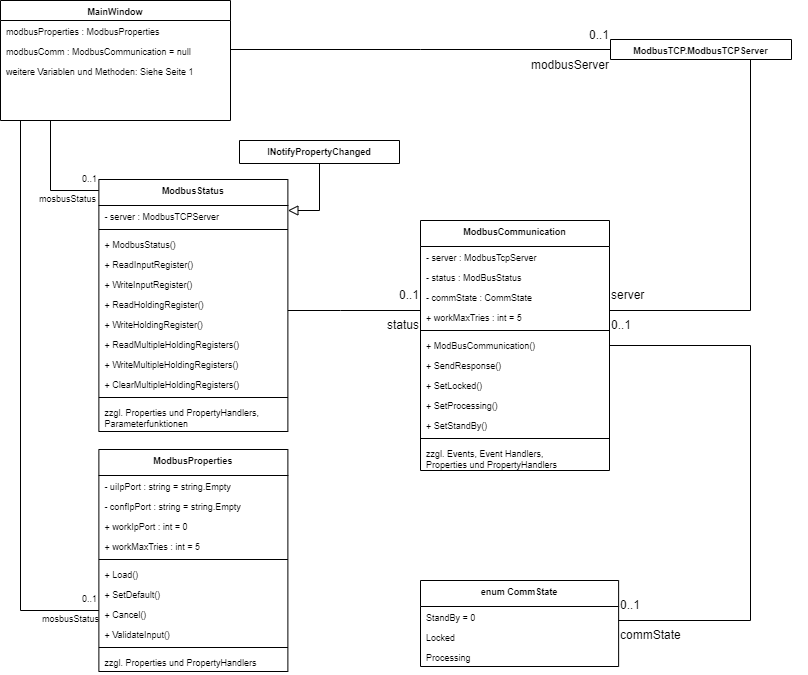
\includegraphics[width = \textwidth ]{Bilder/LV_Klassendiagramm_Modbus}
    \centering
\end{figure}

\subsection{GUI}
Das GUI besteht aus einem Fenster, welches in 8 Bereiche unterteilt ist (siehe Abb.\ref{fig:figure}).
Der Bereich \glqq A\grqq{} hat keine Bedienfunktion.

\subsubsection{ABB Controller Einstellungen}

Der Bereich \glqq B\grqq{} ermöglicht dem Benutzer die Verbindungsdaten zur Steuerung des ABB Roboter IRB140 zu
konfigurieren und die Verbindung herzustellen. 
Die Verbindungsdaten sind voreingestellt und die Felder sind standardmäßig für die Eingabe deaktiviert. 
Die Aktivierung des Felds erfolgt über die Taste \glqq Modify\grqq{}.
Mit der Taste \glqq Save\grqq{} können Änderungen gespeichert werden.

Mit der \glqq Start\grqq{} Taste wird die Verbindung hergestellt.
Die Taste verändert daraufhin ihren Text zu \glqq Connecting...\grqq{} und bei erfolgreich hergestellter Verbindung
zu \glqq Stop\grqq{}.
Ein Symbolbild Informiert dabei über den Verbindungsstatus.

\subsubsection{Modbus Einstellungen}
Im Bereich \glqq C\grqq{} kann der IP-Port des Modbus-Servers über die Taste \glqq Modify\grqq{} angepasst werden.
Direkt nach Programmstart, noch vor der Betätigung der Start-Taste, ist das Symbolbild für den Verbindungsstatus grün
und suggeriert eine erfolgreiche Verbindungsherstellung. 
Nach meinem Verständnis handelt es sich hierbei um eine Fehl-Initialisierung.

Die Verbindungstaste zum Starten der des Automatikbetrieb steht zum Programmstart auf \glqq Stop\grqq{}.

\subsubsection{Produktliste}
Im Bereich \glqq D\grqq{} befindet sich eine scrollbare Liste aller möglichen Produkte mit zwei Spalten.
Es wird neben dem Produktnamen die Produkt-ID angezeigt.
Vermutlich dient die Liste als Nachschlagewerk oder Übersicht, denn es sind ansonsten keine Bedienfunktionen verfügbar.

\subsubsection{Inventaranzeige}
Im Bereich \glqq E\grqq{} Ist die Gleiche Liste um eine Spalte erweitert, in der die gelagerte Menge aufgeführt ist.
Die Liste bildet somit eine bessere Übersicht über das gelagerte Inventar und ist auch als \glqq Inventory\grqq{} gekennzeichnet.
Mit der Checkbox \glqq Show empty entries\grqq{} können Produkte ohne eingelagerte Menge ausgeblendet werden.

\subsubsection{Eventloganzeige}
Bereich \glqq F\grqq{} ist ein Eventlog. Hier werden von dem Programm aus verschiedenste Mitteilungen dem Benutzer angezeigt.
Mit der Taste \glqq clear\grqq{} werden alle existierenden Einträge gelöscht.

\subsubsection{Lagervisualisierung}
Bereich \glqq G\grqq{} ist die Visualisierung des Lagers.
Die drei Reihen \glqq TOP\grqq{}, \glqq MIDDLE\grqq{} und \glqq BOTTOM\grqq{} sollen die drei Regalböden des Lagerregals nachbilden.
Sie sind als hellgraues Rechteck gerendert.

Die Slots A1\ldots A6, H1\ldots H6 sowie H7\ldots H12 sind die Plätze für je eine Palette, die wiederum Platz für
je zwei Becher hat.
Der Ursprung dieser Bezeichnung konnte während der Vorbereitungen auf diese Arbeit nicht geklärt werden.
Wie ich in \ref{Lagerzelle} beschriebe habe, weicht diese Art der Bezeichnung der Lagerplätze von der realen lagerzelle ab.

Das dunkelgraue Rechteck mit der Beschriftung des Lagerorts symbolisiert die Palette.
Die beiden weißen Rechtecke darauf symbolisieren je einen Becher.
Sie sind mit \glqq a\grqq{} für vorne und \glqq b\grqq{} für hinten gekennzeichnet und zeigen den Produktnamen an.

Ist ein Slot für einen Becher leer, wird das entsprechende Rechteck nicht gerendert.
Ein leerer Becher ist ein Produkt im Sinne des Programms.

Ist keine Palette vorhanden, verbleibt der gesamte Bereich der Palette leer.

In der oberen, rechten Ecke kann der Benutzer mit der Checkbox \glqq Show Details\grqq{} zusätzlich die Becher-ID und die
Produkt-ID ein- und ausblenden.

Mit der Checkbox \glqq Edit\grqq{} kann der Benutzer alle Daten (Palette vorhanden/ nicht vorhanden, Becher-ID, Produkt-ID)
als Eingabefeld sehen und ändern.
Der Produktname wird dabei über die Produkt-ID referenziert.
Die Änderungen werden gespeichert, indem die Checkbox einfach wieder abgewählt wird.

\subsubsection{Prozessvisualisierung}

Der Bereich der Prozessvisualisierung ist in der Mitte des Bildschirms.

Im Automatikbetrieb ist dieser grob in 4 Bereiche eingeteilt. 

\textbf{Oben Rechts} ist ein Symbolbild des Industrieroboters IRB 140 dargestellt. 
Das Bild bietet keinerlei Bedienfunktion.

\textbf{Oben links} befindet sich die Start-Taste und im Simulationsbetrieb weitere GUI-Elemente.
Wenn die Verbindungen zum Modbus und zur IRC5-Steuerung hergestellt sind, kann mit ihr der Automatikbetrieb gestartet werden.
Ist der Modbus nicht verbunden, erscheint nach dem Klick ein Dialogfenster.
Der Benutzer wird gefragt, ob aufgrund der fehlenden Verbindung der Controller simuliert werden soll.
Klickt man nun auf \glqq Ja\grqq{}, wird über dem mobilen Roboter ein weiteres Rechteck gerendert.
Es enthält zwei Checkboxen \glqq Mobile Robot is present\grqq{} und \glqq Robot has non-transparent cup\grqq{}.
Erstere rendert nach dem Klick einen mobilen Roboter (schwarzes Oval) und gibt dem Benutzer die Möglichkeit,
wie gewohnt über die beiden Checkboxen im oberen rechten Bereich, Daten eines Bechers und Produkts einzugeben.
Klickt man nun wieder auf die Taste, die nun mit \glqq Stop\grqq{} beschriftet ist, erscheint für etwa eine Sekunde
der Schriftzug \glqq Wait...\grqq{}, bevor das Programm wieder in den Ausgangszustand wechselt.

\textbf{Unten links} befindet sich die Visualisierung des mobilen Roboters. 

\textbf{Unten rechts} befindet sich die Visualisierung des Kommissioniertischs.

Beide Lagerbereiche, für den mobilen Roboter und den Kommissioniertisch,  
geben dem Benutzer die Möglichkeit die Becher- bzw. Produkt-ID ein- und auszublenden oder zu überschreiben.

Weiterhin bietet das Programm keine Möglichkeit den Roboter zu steuern.

\clearpage
\section {Controller}

Der Controller ist eine kleine Anwendung, die die manuelle Bedienung der Lagerzelle ermöglicht.
Die Implementierung der RFID - Funktionen können anhand des Klassendiagramms nicht gezeigt werden.
In Vorbereitung auf diese Arbeit habe ich nicht ausprobiert, ob das Programm diese Funktionen so erfüllt wie sie in dem
GUI impliziert wird.
Für die weitere Arbeit würde dies auch keinen Mehrwert bieten, wie sich in Kapitel \ref{PythonApp}
noch zeigen wird.

\subsection{Klassenstruktur des Controllers}

Der Controller ist genau wie die Lagerverwaltung 3.0 in C$\#$ zusammen mit der .NET-Plattform implementiert.
Da der Controller keinen eigenen Modbus-Server hostet sondern die Klasse \verb|ModbusClient| nutzt, kann er ohne die 
Anwendung \glqq Lagerverwaltung 3.0\grqq{} nicht benutzt werden.

In Abb.\ref{fig:figure6} sieht man, dass das Programm aus zwei wesentlichen Klassen neben dem \verb|MainWindow| besteht.
\verb|ModbusClient| implementiert den Modbus Clienten zur Kommunikation mit den Modbus Servern, die in \ref{ModbusChapter}
beschrieben sind. Die Klasse implementiert auch das in \cite{LarsKistner2017} beschriebene Agentensystem.
\verb|ModbusInfo| dagegen hält die Daten, die zur Erzeugung der Kommandos benötigt werden.

Mit dem Konstruktor der Klasse \verb|MainWindow| werden die Klassen \verb|ModbusClient| und \verb|ModbusInfo| instanziiert.

\begin{figure}
    \caption[Klassendiagramm des Controllers]
    {\small Klassendiagramm des Controllers mit allen vererbenden Klassen, jedoch ohne Klassen die
    lediglich Datentypen konvertieren.}\label{fig:figure6}
    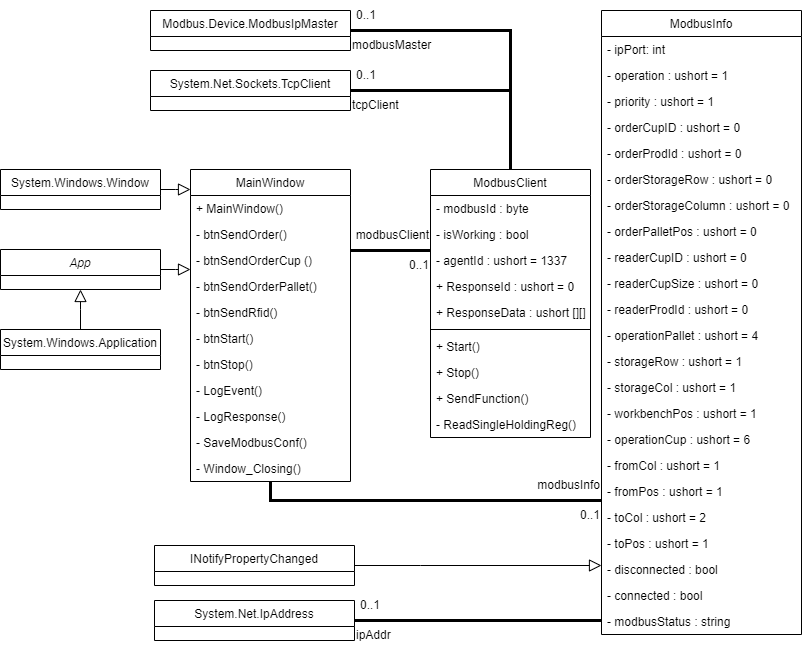
\includegraphics[width = \textwidth ]{Bilder/C_Klassendiagramm}
    \centering
\end{figure}


\subsection{GUI}

\begin{figure}
    \caption[Ansicht des Controller- Startbildschirm ]
    {\small Ansicht des Controller Startbildschirms. }\label{fig:figure5}
    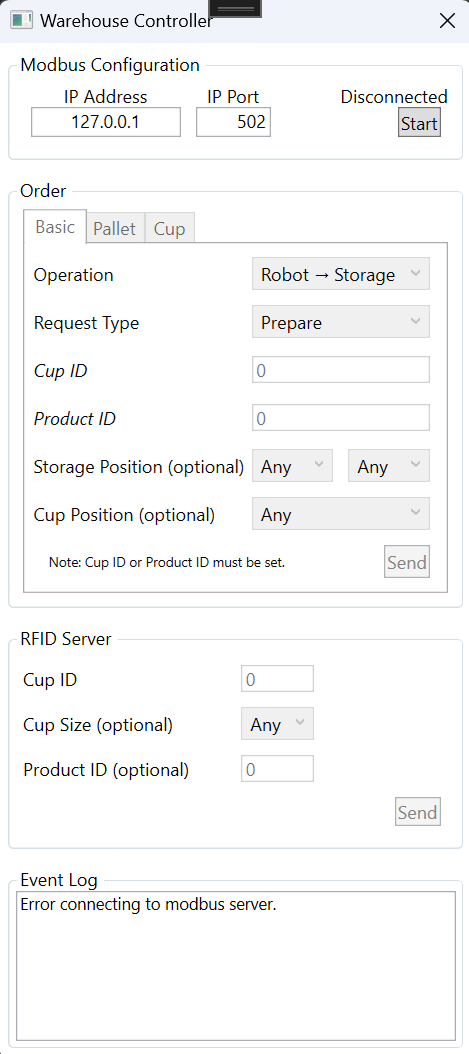
\includegraphics[height = \textheight ]{Bilder/Controller_Startbildschirm}
    \centering
\end{figure}

Wie in \ref{fig:figure5} ersichtlich, ist das Fenster einfach strukturiert und übersichtlich.
Es ist in vier Bereiche unterteilt, die durch eine grau umrandete Box und eine Überschrift abgegrenzt sind.

\subsubsection{Modbus Einstellungen}

Dieser Bereich ist ganz oben und durch die Überschrift \glqq Modbus Configuration\grqq{} gekennzeichnet.
In zwei Textfeldern können Modbus-IP und -Port eingegeben werden. 

Rechts daneben befinden sich untereinander zum Einen ein Label, dass den Verbindungsstatus anzeigt und zum Anderen
ein Knopf mit dem die Verbindung hergestellt und beendet werden kann.

Nach dem Programmstart ist die Beschriftung der Taste \glqq Start\grqq{}.

Mit Klick auf die Taste wird die Verbindung hergestellt und das Label darüber wechselt zu \glqq Connecting...\grqq{}.
Ist die Verbindung erfolgreich hergestellt, wechselt das Label auf \glqq Connected\grqq{} und die Taste wird mit
\glqq Stop\grqq{} beschriftet.

\subsubsection{Kommando erzeugen}

Direkt unter dem Modbus Einstellungsbereich befindet sich der Bereich \glqq Order\grqq{}.
Der Bereich ist durch ein Reitermenü ausgefüllt, dessen Reiter die Überschriften
\glqq Basic\grqq{}, \glqq Pallet\grqq{} und \glqq Cup\grqq{} tragen.

Im Reiter \glqq Basic\grqq{} befinden sich sieben Auswahlfelder und eine Taste.

Mit dem Feld \glqq Operation\grqq{} kann über ein Drop-Down Menü ausgewählt werden, ob ein Becher oder Produkt vom Roboter ins Lager transportiert werden soll oder umgekehrt.

Mit dem Feld \glqq Request Type\grqq{} kann über ein Drop-Down Menü ausgewählt werden, ob der Transport nur Vorbereitet (\glqq Prepare\grqq{}) oder auch ausgeführt (\glqq Execute\grqq{}) werden soll.

Darunter befinden sich Eingabefelder über die die relevante ID (Becher oder Produkt) eingegeben werden kann.

Optional kann darunter über ein Drop-Down Menü die Lagerposition des Lagers oder Bechers ausgewählt werden.


Mit der Taste \glqq Send\grqq{} wird das Kommando an die Steuerung gesendet.

Im Reiter \glqq Pallet\grqq{} kann analog der Transport einer Palette angefordert werden.

Im Reiter \glqq Cup\grqq{} kann analog der Transport eines Bechers angefordert werden.

\subsubsection{RFID Server Tool}

Mit dem RFID Server Tool, dargestellt unter dem Reitermenü, können Speicherblöcke eines RFID-Tags mit der Becher-ID und/oder Produkt-ID
beschrieben werden.
Voraussetzung dafür ist, dass der mobile Roboter mit Becher in der Andockstation des steht.

Die IDs werden in einem Eingabefeld als Zahl eingegeben. Optional kann die Bechergröße ausgewählt werden. 

Mit der Taste \glqq Send\grqq{} werden die Daten auf das RFID-Tag geschrieben.

\subsubsection{Eventlog}

Dies ist ein Textbereich in dem die angeforderten Kommandos aufgelistet werden und eine Mitteilung wenn sie erfolgreich ausgeführt wurden.


\clearpage
\section {RFID Server}

Dieses kleine Programm implementiert einen Modbus TCP/IP Client wie in \ref{ModbusChapter} beschrieben.
Dieser wird genutzt um die gelesenen RFID-Tags für alle Stationen der $\mu$Plant verfügbar zu machen.

In jeder Station der $\mu$Plant gibt es einen RFID Leser der Fa. Feig.

Stationen in der $\mu$Plant können einen Tag am Becher beschreiben wenn sie das Produkt im Becher manipulieren oder die Tags auslesen.
Anschließend können Stationen die einen Becher erhalten, den angekündigten Becher und das Produkt beim Eintreffen
in der Station verifizieren.
Die Verfahren dazu sind in \cite{LarsKistner2017} gut beschrieben.

Die Daten der Tags sollen beim Schreiben und Lesen auf die Modbus Adressen des Modbus Servers geschrieben werden.

Die Auftragswervaltung der $\mu$Plant kann die Daten der Tags dann vom Modbus Server abrufen.
Die RFID-Lesegeräte werden über TCP/IP mittels des SDK der Fa. Feig angesprochen.

\subsection{Klassenstruktur des RFID Servers}

\begin{figure}
    \caption[Klassendiagramm des Programms RFID Server ]
    {\small Klassendiagramm des Programms RFID Server mit allen vererbenden Klassen jedoch ohne solche die
    lediglich Typen konvertieren.}\label{fig:figure8}
    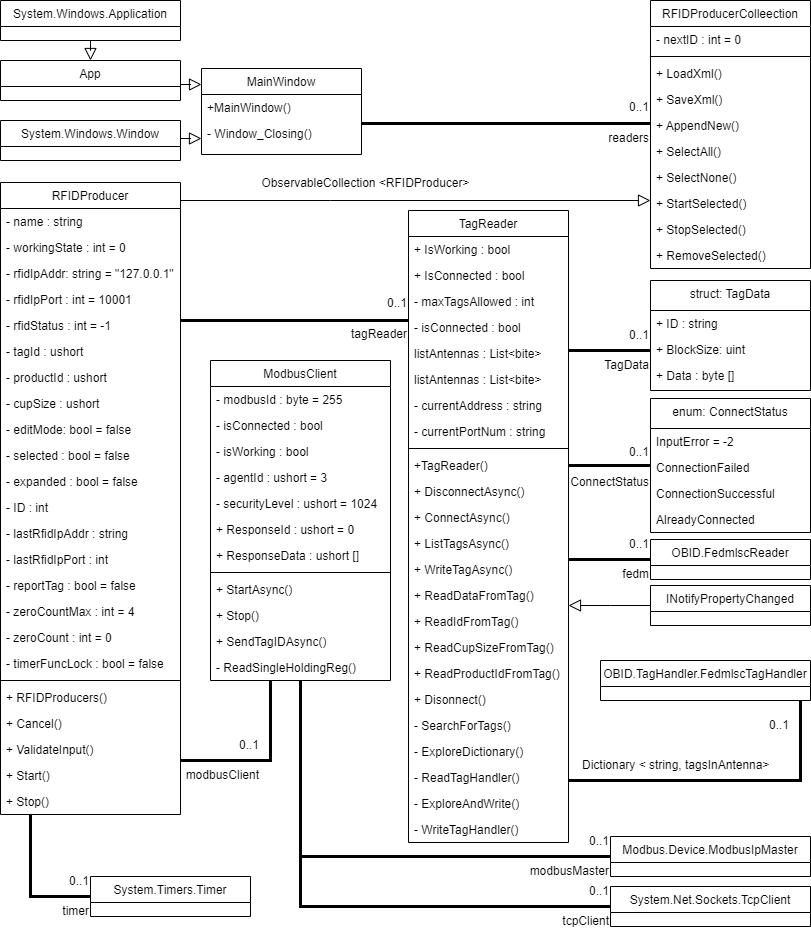
\includegraphics[width = \textwidth ]{Bilder/RFID_Klassendiagramm}
    \centering
\end{figure}

Die Programmstruktur ist anhand des Klassendiagramms in \ref{fig:figure8} erklärt.
Eine Klasse \verb|MainWindow| hält eine Instanz der Klasse \verb|RFIDProducerCollection|.

Diese implementiert die oben beschriebene Liste welche Objekte der Klasse \verb|RFIDProducer| speichert.

Ein \verb|RFIDProducer| Objekt enthält ein Objekt der Klasse \verb|ModbusClient| für die Kommunikation über TCP/IP und
ein Objekt der Klasse \verb|TagReader| für die RFID Kommunikation.


\subsection{GUI}
Das GUI des RFID-Servers ist einfach gehalten und ist in Abb.\ref{fig:figure7} dargestellt.
Das Hauptelement ist eine Liste.
Jedes Listenelement enthält Daten zu einem RFID Modbus Server und einem Tag mit seinen Daten.
Mit der Taste \glqq Add New\grqq{} können neue, leere, Listenelemente erzeugt werden.

Standardmäßig sind die Eingabefelder deaktiviert, können jedoch mit der Taste \glqq Modify\grqq{} zum Bearbeiten
freigeschaltet werden.

Mit der Taste \glqq Start\grqq{} wird die Verbindung hergestellt. Ein Feedback, ob die Verbindung erfolgreich hergestellt
werden konnte ist zunächst nicht ersichtlich.

Jedes Listenelement enthält eine Checkbox mit der es ausgewählt werden kann.

Mit den Tasten \glqq Select All\grqq{} und \glqq Select None\grqq{} können alle Listenelemente an- oder abgewählt werden.

Im unteren, rechten Bereich können mit den Tasten \glqq Start Selected\grqq{} und \glqq Stop Selected\grqq{} mehrere Server
gleichzeitig gestartet und gestoppt werden.

Mit der Taste \glqq Remove Selected\grqq{} können alle ausgewählten Listenelemente gelöscht werden.

\begin{figure}
    \caption[Startbildschirm des Programms RFID-Server]
    {\small Startbildschirm des Programms RFID-Server}\label{fig:figure7}
    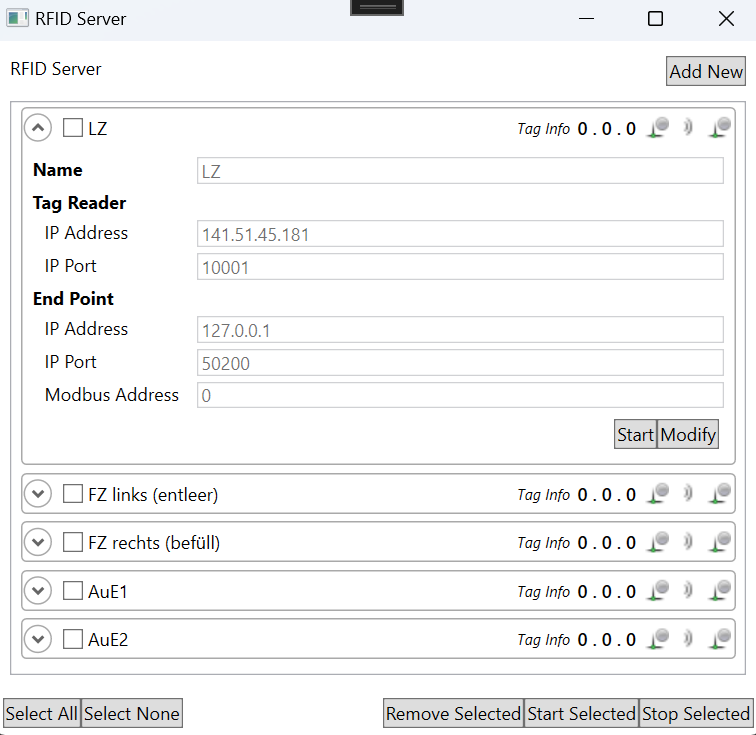
\includegraphics[height = \textwidth ]{Bilder/RFIDServer_Bildschirm}
    \centering
\end{figure}



\newpage
\section{Funktionsanalyse}\label{funktionsanalyse}
In diesem Abschnitt werden die Funktionen der bisher beschriebenen Programme kurz beschrieben und daraus ein gesamter
Funktionsumfang abgeleitet, der für das Kapitel \ref{PythonApp} dienlich sein wird.

\subsection{Lagerverwaltung 3.0}
Dieses Programm hat genau ein Anwendungsfenster welches dem Benutzer einen umfassenden Überblick über die LZ gibt.
Das Fenster hat eine Mindest- und Maximalgröße, ist dazwischen aber beliebig skalierbar. Dialoge werden genutzt, wenn
Einträge gelöscht werden, Verbindungen nicht aufgebaut werden könenn und der Simulationsbetrieb gestartet werden kann.
Felder sind standardmäßig deaktiviert und müssen über Checkboxen aktiviert werden. \\

\subsubsection{Bedienfunktionen}
Der Benutzer kann über das GUI folgende Eingriffe vornehmen:\\
\begin{itemize}
    \item Die Verbindung zu einem Modbus Server konfigurieren, starten und beenden.
    \item Die Verbindung zur ABB IRC5 Steuerung konfigurieren, speichern, starten und beenden.
    \item In der Produktliste kann gescrollt werden.
    \item In der Inventarliste können leere Produkte ein- und ausgeblendet werden.
    \item Die vergangenen Einträge im Eventlogger können gelöscht werden.
    \item In der Lagervisualisierung können an den einzelnen Lagerorten
    \begin{itemize}
        \item Paletten hinzugefügt oder entfernt werden
        \item Becher hinzugefügt oder entfernt werden
        \item Produkt ID und Cup ID der Becher konfiguriert werden
        \item Durch Klick auf einen Becher werden alle Becher gleichen Produkts in der Lagervisualisierung und auch im
        Inventar blau hervorgehoben.
    \end{itemize}
    \item Palette, Becher und Produkt auf dem Kommissioniertisch können konfiguriert werden
    \item Becher und Produkt auf dem mobilen Roboter können konfiguriert werden.
    \item Der Automatikbetrieb kann gestartet werden
    \item Wenn die Verbindung zum Modbus Server nicht hergestellt wurde kann ein Simulationsbetrieb gestartet werden
    \item Im Simulationsbetrieb kann zudem
    \begin{itemize}
        \item Die Anwesenheit eines mobilen Roboters Simuliert werden
        \item ausgewählt werden, dass der Becher auf dem mobilen Roboter nicht transparent ist (Funktion unklar)
    \end{itemize}
\end{itemize}

\subsubsection{Informationsdarstellung}
Der Benutzer wird über folgende Inhalte informiert:\\
\begin{itemize}
    \item Die Verbindungseinstellungen des Modbus Servers und den Verbindungsstatus
    \item Die Verbindungseinstellungen des ABB-Controllers und ihren Verbindungsstatus
    \item Alle möglichen Produkt ID's und die zugehörigen Produktnamen
    \item Produkte und ihre Lagermengen im Inventarbereich.
    \item In der Lagervisualisierung:
    \begin{itemize}
        \item Symbolisierung einer Palette durch dunkelgraues Rechteck, wenn eine Palette vorhanden ist
        \item Symbolisierung der Becher durch weißes Rechteck, wenn ein Becher vorhanden ist
        \item Produknamen und auf Wunsch auch Produkt ID und Becher ID
    \end{itemize}
    \item Im Eventlogger werden folgende Informationen bereit gestellt:
    \begin{itemize}
        \item Fehler und Events der Verbindung über Modbus TCP/IP
        \item Fehler und Events der Verbindung zur Steuerung IRC5 des Industrieroboters
        \item Programmfortschritte und Events im Automatikbetrieb oder der Simulation
    \end{itemize}
\end{itemize}

\subsection{Controller}

Der Benutzer kann folgende Bedienvorgänge durchführen: \\

\begin{itemize}
    \item Die Verbindungseinstellungen des Modbus Servers konfigurieren und starten
    \item Transportbefehle können erzeugt werden:
    \begin{itemize}
        \item Transportbefehle eines einzelnen Bechers zwischen Lager, Kommissioniertisch und Roboter
        \item Transportbefehle für einer Palette zwischen Lager und Kommissioniertisch
    \end{itemize}
    Die beiden Befehle können einerseits direkt ausgeführt werden, andererseits können sie auch als Eingabe für die
    Lagerverwaltungssoftware benutzt werden.
    \item Ein Becher in der Andockstation kann mittels einem RFID- Lesegerät beschrieben werden.
\end{itemize}

Der Benutzer wird in diesem Programm nur über seine Eingaben Informiert.
Die Eingaben erfolgen wo möglich über ein Dropdown Menü

\subsection{RFID Server}

Der Benutzer kann folgende Bedienvorgänge durchführen: \\

\begin{itemize}
    \item Einen Neuen Listeneintrag erzeugen
    \item Einen oder alle Listeneintrag markieren
    \item Markierte Listeneinträge abwählen
    \item ausgewählte Listeneinträge Löschen, Verbindung starten oder stoppen
    \item Je Listeneintrag kann der Benutzer folgende Einstellungen vornehmen:
    \begin{itemize}
        \item IP und Port des Tag Readers
        \item IP, Port und Modbus Adresse des Endpoints
    \end{itemize}
    \item Ein einzelner Listeneintrag kann gestartet werden
    \item Mit der Taste \glqq Modify \grqq kann ein Listeneintrag zum Bearbeiten freigeschaltet werden
    \item Mit der Taste \glqq Save \grqq können Änderungen gespeichert werden.
\end{itemize}

Der Benutzer sieht in diesem Programme eine Liste aller eingetragenen RFID Reader, Endpoints und Modbus Adressen.
Jeder Listeneintrag kann auf eine Zeile minimiert werden die lediglich den Namen des Endpunkts und die gelesenen
Tag Daten anzeigt.
Im ausgeklappten Zustand sind die Konfigurationen sichtbar, aber grau hinterlegt um anzudeuten, dass die Bearbeitung
gesperrt ist.


